\chapter{Dark Matter at IceCube}\label{chap:neutrinos}

The existence of a mass for the SM neutrino is a puzzle within the vanilla $\rm{SU}(3) \times \rm{SU}(2) \times \rm{U}(1)$ picture of particle physics. As such, it provides an interesting technical challenge to build extensions to the SM that solve this problem. Of interest in this Chapter is an effective theory which contains a stable Dark Matter candidate as well as radiatively generating neutrino masses. We consider the effect of such a model on the propagation of neutrinos across the Universe. In particular we look at how the mean free path is modified, and compare this to sources identified at the IceCube neutrino observatory. We use this to place limits on parameters in the model which are competitive and complementary to those from cosmology, astrophysics, and collider searches.

\section{How to Generate a Neutrino Mass}


In the neutrino sector, there are two possible types of mass term in the Lagrangian \cite{Ma1998, Bellini2018, Boehm2006, Yao2018};
\begin{itemize}
  \item \textit{Dirac Neutrino Masses} arise after the introduction of a right-handed neutrino field $\nu^i_R$ with $i = e, \mu, \tau$. The mass then arises under the Higgs mechanism due to a coupling;
  \begin{equation}
    \mL_{\textrm{\small lept}, \phi} \propto \lambda^{ij}\bar{\psi}^i\Phi\ell^j + \lambda_\nu^{ij}\bar{\psi}^i\Phi^c \nu^i_R
  \end{equation}
  where $\psi^i$ is the left handed $\rm{SU}(2)$ lepton doublet, $\Phi$ is the $\rm{SU}(2)$ Higgs doublet, and $\ell^j$ is the right-handed lepton singlet. After electroweak symmetry breaking (EWSB), the neutrinos get a mass term;
  \begin{equation}
    -\sum_{i}{m_\nu^i \left(\bar{\nu}^i_R \nu^i_L + \bar{\nu}^i_L \nu^i_R\right)}
  \end{equation}
  \item \textit{Majorana Masses} are a qualitatively different scenario that is possible if the fermion is neutral, as in the case of the neutrino. In this case, the right-handed neutrino field is not independent of the left-handed one.\footnote{To be precise, $\nu_R(x) =
  \nu_L^c(x)$ where $c$ represents the charge conjugated field.} The mass term becomes;
  \begin{equation}\label{eq:Majorana Mass Term}
    -\frac{1}{2}\sum_{i}{m_\nu^i \left(\bar{\nu}_L^{i,c}\nu_L^i + \bar{\nu}^i_L \nu^{i, c}_L\right)}
  \end{equation}
\end{itemize}
We will focus on the second scenario. This can't arise at tree level in the Standard Model. The lowest dimension for which such a term is generated is at dimension $5$ via an operator of the form \cite{Bonnet2012};
\begin{equation}
  \Lambda^{-1}\phi^0 \phi^0 \nu^i_L \nu^j_L
\end{equation}
Being dimension $5$, the operator is not renormalisable, and as such this can only be an effective coupling, valid up to some large mass scale $\Lambda$.

\section{The Low Energy Effective Field Theory}

The discussion of UV complete theories \cite{Farzan2009, Farzan2010, Farzan2010a} presents a concrete scenario to implement the ideas of radiatively generating neutrino mass, as well as providing a dark matter candidate. On the other hand, at a given low energy scale, our experiments will not be able to probe the UV structure of the theory, only the effective degrees of freedom remaining at the scale in question (e.g. the energy scale at the LHC, or in cosmological scenarios).

In this section, we will present a low energy effective theory that contains a scalar Dark Matter candidate coupled to neutrinos. This was originally proposed in \cite{Farzan2014, Farzan2011, Farzan2010, Boehm2006, Farzan2009}. A key distinction will be between real and complex scalar Dark Matter, since the two have qualitatively different constraints. We will focus on the phenomenological consequences of the model and be as clear as possible as to exactly what constraints these place on the couplings and masses within the theory. These include astrophsyical, particle physics, and cosmological bounds \cite{Farzan2014, Farzan2011, Farzan2010, Boehm2006, Farzan2009}. To see how the model radiatively generates neutrino masses, see Appendix \ref{sec:neutrinomass}.

It is not within the scope of this work to present a full UV completion of this effective theory. Nonetheless, \cite{Farzan2009, Farzan2010} present such a completion in the real case. In \cite{Farzan2010a} the same is done for complex dark matter. The fact that the particle content of the effective model can arise from a fully gauge invariant theory is important since it provides a clear understanding of where the relevant degrees of freedom come from, as well as the scale of new physics.

\subsection{Lagrangian and Particle Content}

Our focus is on a low energy particle spectrum that consists of the Standard Model along with \cite{Farzan2014, Farzan2011};
\begin{itemize}
  \item A scalar field, $\delta$, which may be real or complex;
  \item Two or more massive right-handed fermions $N^i_R$, in what follows, we will assume these to be of \textit{Majorana} type.
\end{itemize}
In addition to this, we assume that there is a residual $\mathbb{Z}_2$ symmetry \cite{Ma1998, Ma2001, Ma2006} under which the new particles are odd, and the Standard Model is even. This has a number of effects;
\clearpage
\begin{enumerate}
  \item It ensures that the lightest particle in the spectrum is stable, providing a Dark Matter candidate.
  \item It prohibits a term of the form $\phi^0 \bar{N}_R^i \nu^\alpha_L$, so that after EWSB, there is no Dirac mass term linking $N^i_R$ and $\nu^\alpha_L$. This means that the neutrino mass is not generated at tree level.
  \item The new scalar, $\delta$, cannot acquire a VEV, due to the structure of the Higgs sector.
\end{enumerate}
The key feature we are interested in however is the interaction part of the Lagrangian which couples this new dark sector to the neutrino sector in the Standard Model. In our effective theory, we take the couplings to be of the form;
\begin{equation}\label{eq:effective lagrangian}
  g_{i\alpha}\delta \bar{N}^i_R \nu^\alpha_L + \text{h.c.}
\end{equation}
\noindent Where there is an implicit sum over the right-handed fermion species, $i$, and the Standard Model neutrino species, $\alpha$. Later we will be interested in constraining the values of the coupling constants. To see the explicit contributions to the neutrino mass see Appendix \ref{sec:neutrinomass}. 

\subsection{Astrophysical, Cosmological, and Particle Physics Constraints}




So far we have illustrated (i) how neutrino mass is generated within the effective framework, and, (ii) discussed which are the relevant degrees of freedom when it comes to suitable dark matter candidates. We now discuss the vital question as to what constraints have already been placed on the model across a range of scenarios. We will investigate the constraints that arise from the two key scenarios \cite{Boehm2006, Franarin2018, Farzan2009, Farzan2011, Farzan2014, Farzan2010};
\begin{enumerate}
  \item The cosmological bound on the Dark Matter annihilation cross section;
  \item The bounds that arise due to light meson and tau decay.
  \item Bounds that arise from observations of the CMB and Big Bang Nucleosynthesis (BBN)
\end{enumerate}
For completeness, we will also discuss some of the other astrophysical bounds in slightly more general terms.
\subsubsection{Dark Matter Annihilation Cross Section}
Within this effective model, there are three annihilation channels in the case that $N^i_R$ is a Majorana fermion, given by $\delta \delta \rightarrow \{\nu\nu, \nu\bar{\nu}, \bar{\nu}\bar{\nu}\}$. As in \cite{Boehm2006}, we take $\Lambda \sim 200 \, \text{GeV}$, $0.01 \, \text{eV} < m_\nu < 1\, \text{eV}$. Furthermore, we also use the fact that sub-GeV Dark Matter requires $\langle \sigma v \rangle \simeq 5 \times 10^{-26}\, \text{cm}^3\text{s}^{-1}$ in order for the correct relic abundance to be obtained \cite{Steigman2012}.

\vspace{-0.3cm}

\subsubsection*{Real Scalar Dark Matter}
In the real case, this gives the constraints;
\begin{equation}
  \mathcal{O}(1 \, \text{MeV}) \lesssim m_\delta < m_N \lesssim 10 \, \text{MeV}, \quad 3 \times 10^{-4} \lesssim g \lesssim 10^{-3}
\end{equation}
\noindent This is a strong bound on the coupling, and in fact we can \emph{only} obtain new constraints in the complex case. The real case is too weakly coupled. From now on therefore, whilst we will of course mention the real case, our focus will be on the complex scenario.

\vspace{-0.3cm}

\subsubsection*{Complex Scalar Dark Matter}
In the complex case \cite{Boehm2006}, we get less stringent constraints on the masses;
  \begin{equation}
    (1\, \text{MeV})^2 \lesssim \left|m_{\delta_2}^2 - m_{\delta_1}^2\right| \lesssim (20 \, \text{MeV})^2
  \end{equation}
\noindent We note that now $m_N$ is a free parameter, so is far less constrained than in the real case. In turn, this implies that $g$ is less constrained, although we shall see that there are different bounds due to light meson decay.

\vspace{-0.3cm}

\subsubsection{Light Meson and Tau Decay}


Consider the decay $K^+ \rightarrow e^+/\mu^+ + \nu$ \cite{Farzan2011, Farzan2014, Farzan2010}. Then generically if the coupling in \eqref{eq:effective lagrangian} is present, new decay modes $K^+ \rightarrow e^+/\mu^+ + N^i_R + \delta$ should exist. This means we should see $K^+ \rightarrow e^+/\mu^+ + \text{missing energy}$ compared to the Standard Model. This can be tested by experiments such as KLOE. Importantly, in this case the bounds are valid in the real \emph{and} complex scenarios. They are presented in \cite{Farzan2011, Farzan2014, Farzan2010, Artamonov2016};
  \begin{equation}
    \sum_{i}{\Abs{g_{ie}}^2} < 10^{-5}, \quad \sum_{i}{\Abs{g_{i\mu}}^2} \lesssim 10^{-4}, \quad \sum_{i}{\Abs{g_{i\tau}}^2} < 10^{-1}
  \end{equation}
\noindent There are a couple of important observations that need to be made with respect to these bounds;
\begin{itemize}
  \item Provided $\max(m_\delta, m_{N^i}) \ll m_{K, \pi} \simeq \mathcal{O}(500\,\text{MeV})$, the bounds are similar in both the complex and the real case;
  \item With the bounds as above, we note that the couplings themselves can have magnitudes;
  \begin{equation}
    \label{eq:constraints}
    \Abs{g_{ie}} \lesssim 3 \times 10^{-3}, \quad \Abs{g_{i\mu}} \lesssim 10^{-2}, \quad \Abs{g_{i\tau}} \lesssim 3 \times 10^{-1}
  \end{equation}
  \item In the heavy case \cite{Farzan2014}, $m_K < m_\delta + m_{N^i} < m_D$, where $m_D$ is the mass of the $D$ meson, the bounds above do not apply. Instead the strongest bounds have $\Abs{g_{ie}} \lesssim 0.4$ and $g_{i\mu} \lesssim \mathcal{O}(1)$.
\end{itemize}

\subsubsection{CMB Constraints on the Scalar Mass}\label{sec:cmbconstraints}

There are additional constraints on light particle dark matter that arise from measurements of the CMB, the light element abundance, and the expansion rate of the Universe. They apply here because, firstly, the existence of a light species such as our dark matter candidate during BBN at $z \sim 3 \times 10^8$ could change the rate of expansion and hence the time of weak freeze-out, changing relic abundances. Secondly, additional energy might be injected into the neutrino sector as this dark matter candidate annihilates. The relevant constraints are shown in Table \ref{tab:cmb} and are based on \cite{Boehm}, \cite{Nollett2015}, and \cite{Escudero2019}.

\begin{table}[t]
\centering
\begin{tabular}{lcc}
\toprule \textbf{Constraint} & \textbf{Mass Bound [MeV]} & \textbf{Min. Neutrino Energy [PeV]} \\
\midrule 
$N_{\textrm{\small eff}}$ \cite{Boehm} & 3.90 & 0.76 \\
BBN + Planck + $N_{\textrm{\small eff}}$ + $Y_p$ \cite{Nollett2015} & 6.74 & 2.27 \\
BBN + Planck + $N_{\textrm{\small eff}}$ \cite{Nollett2015} & 6.98 & 2.43 \\
Planck + BAO + $H_0$ + $N_{\textrm{\small eff}}$ \cite{Escudero2019} & 7.80 & 3.04 \\
\bottomrule
\end{tabular}
\caption{Table illustrating the constraints on complex scalar dark matter coming from various cosmological sources as well as the corresponding minimum neutrino energy that would need to be observed to probe parameter space outside of these bounds.}
\label{tab:cmb}
\end{table}

Kinematically, the constraints are relevant in this scenario because the centre of mass energy of the $\nu\nu \rightarrow \delta\delta$ interaction determines the maximum mass $m_\delta$ of the scalar particle that can be produced;
\begin{equation}
    m_\delta \leq \frac{1}{2}\sqrt{s} = \frac{1}{2}\sqrt{2 E_\nu m_\nu}
\end{equation}
where $E_\nu$ is the energy of the high-energy neutrino from the blazar. We see therefore that the CMB bounds on the mass of the scalar are related to a minimum neutrino energy above which the method set out in this paper will probe parameter space unconstrained by the CMB, although we note this is not quite the case for the currently observed event. Stated another way the fact we are only sensitive to MeV scale dark matter is partly due to the centre of mass energy for the $\nu\nu \rightarrow \delta\delta$ interaction being less than the threshold energy for larger scalar masses.  The $290$ TeV neutrino is not at the upper end of the expected blazar neutrino flux distribution, so it is not unreasonable to expect that higher energy neutrinos will be observed, immediately allowing us to probe higher mass regimes, less sensitive to CMB constraints. To investigate this quantitatively, we choose $m_\nu = 0.04\,\mathrm{eV}$ to be the lightest neutrino species. This ensures that $\sum{m_\nu} < 0.17 \, \mathrm{eV}$. Then, for each bound we may compute the minimum neutrino energy that must be observed to probe new parameter space. These reference neutrino energies are also shown in Table \ref{tab:cmb}. We consider how this maps onto the expected constraints that would be obtained with observations of higher energy neutrinos in Figure \ref{fig:mpmn}.

As a final comment, there is work being done currently that re-explores some of the assumptions in deriving these constraints based on entropic or decay arguments, see for example \cite{Kreisch}. Figure 3 in \cite{Wilkinson} proves a useful reference to see the separate constraints from BBN and the CMB. With this in mind, we view the bounds presented in this paper as complementary to those from Cosmology, requiring different (in this case astrophysical) assumptions.

\subsubsection{Additional Constraints}



The two methods of constraining the effective theory given above provide the most stringent bounds on the couplings and the masses. Furthermore, they also provide two very distinct scenarios for comparison. The first investigates the phenomenology in the setting of thermalizing early universe cosmology, whilst the second is a pure particle physics test. Within the literature \cite{Farzan2010, Boehm2006}, there are a couple of other suggestions for additional, or future methods of constraint. These include;
\begin{enumerate}
  \item \textit{Supernova Core Collapse:} It is suggested \cite{Franarin2018, Farzan2010} that we could search for a dip in the neutrino energy spectrum coming from neutrinos produced during supernova core collapse.
  \item \textit{Large Scale Structure:} This places constraints on the mass \cite{Boehm2004} due to the damping length of $\mO(\text{keV}) \lesssim m$.
\end{enumerate}
\subsection{$\nu\nu \rightarrow \delta\delta$ Cross-Section}\label{sec:crosssection}
We are interested in the processes of the form;
\begin{align*}
\nu \,\, \nu &\longrightarrow \delta \,\, \delta\\
\nu \,\, \overline{\nu} &\longrightarrow \delta \,\, \delta
\end{align*}
If the neutrinos are Majorana, both of these processes can occur and the cross-section is given by;
\begin{multline}
\label{eq:sigma}
\sigma(s) = \frac{g^4 m_N^2}{32 \pi}\left[\sqrt{\frac{\frac{1}{4}s - m_\delta^2}{s}}\frac{2}{\left(m_\delta^2 - m_N^2 - \frac{1}{2}s\right)^2 - s\left(\frac{1}{4}s - m_\delta^2\right)} \right. \\ \left. + \frac{1}{s\left(m_\delta^2 - m_N^2 - \frac{1}{2}s\right)}\log\left(\frac{m_\delta^2 - m_N^2 - \frac{1}{2}s + \sqrt{s\left(\frac{1}{4}s - m_\delta^2\right)}}{m_\delta^2 - m_N^2 - \frac{1}{2}s - \sqrt{s\left(\frac{1}{4}s - m_\delta^2\right)}}\right)\right]
\end{multline}

\vspace{-1cm}

\section{IceCube, IceCube 170922A and TXS 0506+056}

The IceCube neutrino observatory \cite{IceCube} is located at the South Pole, consisting of one cubic kilometre of Antarctic ice. The goal of the project is to detect very high energy neutrinos from astrophysical sources. In this regard it is sensitive to energies in the range $300\,\text{GeV}$ to $1\,\text{EeV}$. The important specifics of the design are that it is a Cherenkov detector. When a muon neutrino interacts with the ice via charged current interactions, a muon is produced which emits Cherenkov radiation as it propagates through the medium. The energy of this muon, $\hat{E}_\mu$ is measured along with the propagation path. This can then be used to reconstruct;
\begin{itemize}
  \item The neutrino energy $E_\nu$, from the muon energy prior, $\hat{E}_\mu$ via for example Figure S5 in \cite{IceCube2018}. As a reference, in \cite{Kelly}, an estimated fit is given which can be used in simple practical cases;
  \begin{equation}
    \left(\frac{E_\nu}{\textrm{TeV}}\right) = 1.92\left(\frac{\hat{E}_\mu}{\textrm{TeV}}\right)^{1.14}
  \end{equation}
  \item The declination and right ascension of the original neutrino path.\footnote{One can access this data \href{https://icecube.wisc.edu/science/data/access}{\textit{here}}.} This is vital in matching up events with possible sources, and has lead to the deduction that the neutrino events we will be interested were most likely sourced from a blazar, TXS $0506$+$056$, at a redshift of $z \simeq 0.3365$.
\end{itemize}

\noindent The IceCube experiment is searching for high energy astrophysical neutrinos. Only very particular types of astrophysical object can produce such energetic particles. Of particular interest to us are objects known as \textit{blazars}. These are \textit{Active Galactic Nuclei (AGN)}, which consist of a supermassive black hole that converts the gravitational and rotational energy of accreting matter into highly relativistic jets \cite{Ackermann2018} pointing in our direction. In particular, IceCube believes to have detected high energy neutrinos from a known $\gamma$-ray source TXS $0506$+$056$. The key fact regarding this blazar is that it is at a redshift \cite{Kelly};
\begin{equation}
  z_{\mathrm{TXS}} \simeq 0.3365 \Rightarrow d_{\mathrm{TXS}} \simeq 1.3 \, \textrm{Gpc}
\end{equation}
\noindent where $d_{\mathrm{TXS}}$ is the comoving distance to the blazar.\footnote{$1\,\textrm{Gpc} \simeq 3.08567 \times 10^{27} \, \textrm{cm}$} This therefore presents a very interesting regime in which to test fundamental physics: we have $\textrm{TeV}$ - $\textrm{PeV}$ energy neutrinos propagating across gigaparsecs of distance. Along the way, we can therefore consider interactions with dark matter, the cosmic neutrino background etc. As we shall discuss further below, it also presents a prime example of the utility of \textit{multimessenger astronomy} \cite{Kelly, Ackermann2018} where neutrino events are calibrated with other $\gamma$ and X-ray experiments such as Fermi-LAT, H.E.S.S., and the Swift XRT.

To understand the relationship between the flaring $\gamma$-ray source TXS $0506$+$056$ and IceCube, one should note that on $22$ Septemeber $2017$, a neutrino with an energy of $\sim 290\,\textrm{TeV}$ was observed at IceCube (IceCube-170922A). This prompted a couple of responses;
\begin{itemize}
  \item \textit{Multimessenger Approach:} Immediately after the event, multiple collaborations began to establish the coincidence of the neutrino alert with the flaring state of TXS $0506$+$056$. Broadly this relies on correlating $\gamma$-ray and X-ray measurements of known catalogs of astrophysical objects with the angular position of the reconstructed neutrino path. For a more detailed account of this, see \cite{Ackermann2018}, however the salient point is that the chance coincidence is currently ruled out at $3-3.5\sigma$.
  \item \textit{Historical Approach:} It also provoked a search into data taken in $2014-15$ where it was found that $13 \pm 5$ excess events \cite{Kelly} appear to \textit{also} be coincident with TXS $0506$+$056$ in its flaring state. It thus appears that this blazar is a source of high energy astrophsyical neutrinos.
\end{itemize}
We will be interested in the high energy event to place our own constraints on the model under consideration. The careful analysis in \cite{Ackermann2018} provides a most probable energy of $290 \, \textrm{TeV}$ with a $90\%$ confidence level lower bound of $183 \, \textrm{TeV}$. More information on the analysis of the coincidence of IceCube-170922A with the flaring of TXS $0506$+$056$ as well as the historical data can be found in \cite{Ackermann2018, IceCube2018, Kelly, Padovani2018}. Furthermore, the viability of blazars as neutrino sources is discussed in \cite{Hooper2018, IceCube2018}.


\subsection{The Neutrino Luminosity from TXS 0506+056}\label{sec:nuluminosity}


We intend to use the mean free path, which we can define via;
\begin{equation}
  \ell^{-1} = \sum_{i}{n_{X_i} \sigma(\nu X_i \rightarrow Y_i)}
\end{equation}
to place bounds on the model. In order to use the observation of the $290 \, \textrm{TeV}$ neutrino as a constraint on fundamental interactions within the dark and neutrino sectors, we first must discuss the validity of comparing the mean free path to the comoving distance from the blazar. If the neutrino luminosity associated to the blazar is of a magnitude that saturates the maximum bound, we may deduce that the mean free path of the neutrinos is likely to be \textit{larger} than the comoving distance. To do so, we extract the 7.5 year upper bound on the neutrino luminosity as given in Figure 4 of \cite{Ackermann2018}. Referring to $1.7$ in \cite{dermer2009high}, the \textit{luminosity} radiated by a source between energies $\epsilon_1$ and $\epsilon_2$ is then simply;
\begin{equation}
  L[\epsilon_1, \epsilon_2] = 4\pi d_L^2 \int_{\log \epsilon_1}^{\log \epsilon_2}{\upd{\log\epsilon} \nu F_\nu }
\end{equation}
where $d_L$ is the photometric distance to the source. This upper bound is shown in Table \ref{tab:luminosity} along with the upper bound provided by the HAWC experiment on the photon flux. It should be emphasised that the main comparison point here is the neutrino luminosity, not the photon luminosity which is given to provide support for a given production mechanism. The value for the photons does not affect the conclusions regarding the bounds on the neutrino couplings. The inclusion of the photon flux will be discussed further in the next section. To proceed, we compare the neutrino luminosity with upper bounds derived in blazar modelling scenarios, in particular those given in \cite{Padovani2019}. Other references which make a detailed record of the relevant production mechanisms inside the jet environements of the blazar include \cite{Gao2018nat, Rodrigues2018, Padovani2018, Keivani2018}. 
\begin{table}[t]
\centering
\begin{tabular}{p{3.0cm}p{3cm}p{4cm}p{3.5cm}p{2.0cm}}
\toprule \textbf{Source} & \textbf{Energy Range} & \hfill \textbf{Luminosity} $\text{erg}\,\text{s}^{-1}$ & \textbf{Reference}\\
\midrule
\textit{Neutrino Source} & $186 \, \textrm{TeV}$ - $7.9 \, \textrm{PeV}$ & \hfill $\lesssim 10^{46}$ & \cite{Ackermann2018} \\
\textit{$\gamma$ Source (HAWC)} & $0.8 \, \textrm{TeV}$ - $74.0 \, \textrm{TeV}$  & \hfill $\lesssim 4.1 \times 10^{45}$ & \cite{Ackermann2018, HAWC} \\
\bottomrule
\end{tabular}
\caption{Numerical Results for the luminosity in the given energy range for the $\gamma$-ray and neutrino components of the blazar flux. Note that in the neutrino case, we are considering the 7.5 year exposure presented in \cite{Ackermann2018}}
\label{tab:luminosity}
\end{table}
We make the following observations. It might appear that there is a conflict between the upper bound of $\sim 10^{45} \,\textrm{erg}\,\textrm{s}^{-1}$ in \cite{Padovani2019} and that presented in Table \ref{tab:luminosity}. There are two reasons this is not the case;
\begin{enumerate}
    \item The value quoted in Table \ref{tab:luminosity} is an upper bound on the measurement due to the fact that an ensemble of distant sources may lead to a neutrino observation even if the expectation value for one source is very small \cite{Padovani2019}.
    \item The value quoted in \cite{Padovani2019} assumes that there is only one emmiting region within the blazar jet. Other studies such as \cite{Murase2014} find luminosities that saturate this upper bound due to multiple emitting regions.
\end{enumerate}
With this in mind, the data is consistent with the different theoretical predictions for the expected neutrino luminosity. Up to the uncertainty in this modelling, it appears that the measured luminosity is indeed close to saturating this bound. We then make a key deduction of this work, that therefore the mean free path of the 290 TeV neutrino is likely to be greater than the distance to the blazar. This will be the definition of our bound. For a discussion regarding the consistency of the neutrino and photon flux, see Appendix \ref{sec:consistent}.

\section{Results}

There are a number of motivated assumptions that go into deriving the following constraints regarding the neutrino mass hierarchy, neutrino mass eigenstates, the redshift of the neutrino energy as it propagates across the Universe, and the contribution of other channels. This is detailed in Appendix \ref{sec:assumptions}. Before presenting the results, we discuss the methodology applied, in particular what parameter space we explore, and which effects are included in the analysis. For a given set of parameters ($g_{ie}, \cdots, m_\delta, m_N$), the approach taken is as follows;
\begin{enumerate}
  \item Consider the scattering of a $290 \, \textrm{TeV}$ muon-neutrino off the mass eigenstates in the cosmic neutrino background.
  \item Compute the cross-section at the centre of mass energy \emph{for each} mass eigenstate. This allows us to include the different neutrino hierarchies.\footnote{In the complex case, we include an additional factor of $3$ as discussed in Section \ref{sec:complexsplit}}
  \item Compute the mean free path, including the redshifting effect and compare to the distance to the blazar.
  \item Reject parameters sets for which the mean free path is less than this distance.
\end{enumerate}

\subsection{Parameter Choices}


In terms of the parameters we choose, we are informed by the current leading observational bounds on (i) the total neutrino mass, and, (ii) the coupling constants in the effective theory. Before proceeding, we make it clear that we could not improve on the constraints $g_{\ell} \lesssim 10^{-3}$ in the case of real dark matter. The mean free path was always significantly larger than the distance to the blazar. All the results that follow are in the complex case, where for example, the coupling to the tau neutrino is far less constrained. Taking the constraints from \eqref{eq:constraints}, we choose the following for our computations;
\begin{itemize}
  \item The mean free path is most sensitive to the coupling, $g_{i\mu}$, as such we choose to vary this parameter in the range $g_{i\mu} \in [10^{-5}, 10^{-1}]$.
  \item We also vary the mass of the mediator $m_N \in [m_\delta, 10\,\textrm{MeV}]$.
  \item We fix the mass of the scalar $m_\delta$ for values $m_\delta = 0.1, 0.5, 1.0, 1.5 \, \textrm{MeV}$.
  \item The electron neutrino coupling is the most constrained, and indeed we find that the conclusions are insensitive to this parameter. As such, we set $g_{ie} = 0$, removing the dependence.
  \item In all the plots below we have take $g_{\tau} = 3\times 10^{-1}$, at the upper bound of the current constraints. We acknowledge that this may be slightly optimistic.
  \item Finally we consider values of the lightest neutrino (in both hierarchies) of $m_\nu = 0.01, 0.03, 0.04\,\textrm{eV}$. All of these values are within the Planck bound of $\sum_{\nu}{m_\nu} < 0.17 \, \textrm{eV}$. Although, since this bound appears to be getting tighter, the lower neutrino masses e.g. $m_\nu = 0.01 \Rightarrow \sum_{\nu}{m_\nu} \simeq 0.06 \, \textrm{eV}$ perhaps lead to stronger conclusions.
\end{itemize}


\subsection{Analysis}
A selection of results are shown in Figure \ref{fig:main} across a range of neutrino and scalar masses. For a complete set of plots, the reader should consult \cite{Alvey:2019jzx}. Note that the shaded regions in each figure are those that are ruled out by the mean free path, relic abundance, and kaon decay constraints. For example, masses of the mediator above $10 \, \textrm{MeV}$ are ruled out by the thermal cross-section calculations.

\noindent As we will discuss shortly, the constraints we obtain in this way are stronger than those from Kaon decays, but slightly weaker than the constraints from BBN and CMB, we shall discuss this in more detail very shortly.  We see from the plots that at low mediator masses $m_N \lesssim 5\, \textrm{MeV}$, we see a big improvement over the kaon decay constraints. Indeed in the $m_\delta = 0.1\,\textrm{MeV}$ scenario, we see an order of magnitude improvement across a decent range of mediator masses. There is also not a strong dependence on the neutrino masses. This suggest that even if the cosmological bounds on the total sum of neutrino masses tightens, these constraints will not weaken significantly. Furthermore, whilst there is a slight difference between the neutrino hierarchies due to the different couplings to the mass eigenstates, this is again not significant. Hence, we are not sensitive to future revelations from the neutrino sector.

In addition, we have also neglected additional processes that would decrease the mean free path. These include $\nu\delta \rightarrow \nu\delta$. As discussed in Section \ref{sec:oneprocess}, we do believe that this will be a negligble contribution. Nonetheless, again the conclusions are insensitive to this. This is because any decrease in the mean free path would only \emph{strengthen} the constraints.

\begin{figure}[t]
 \centering
 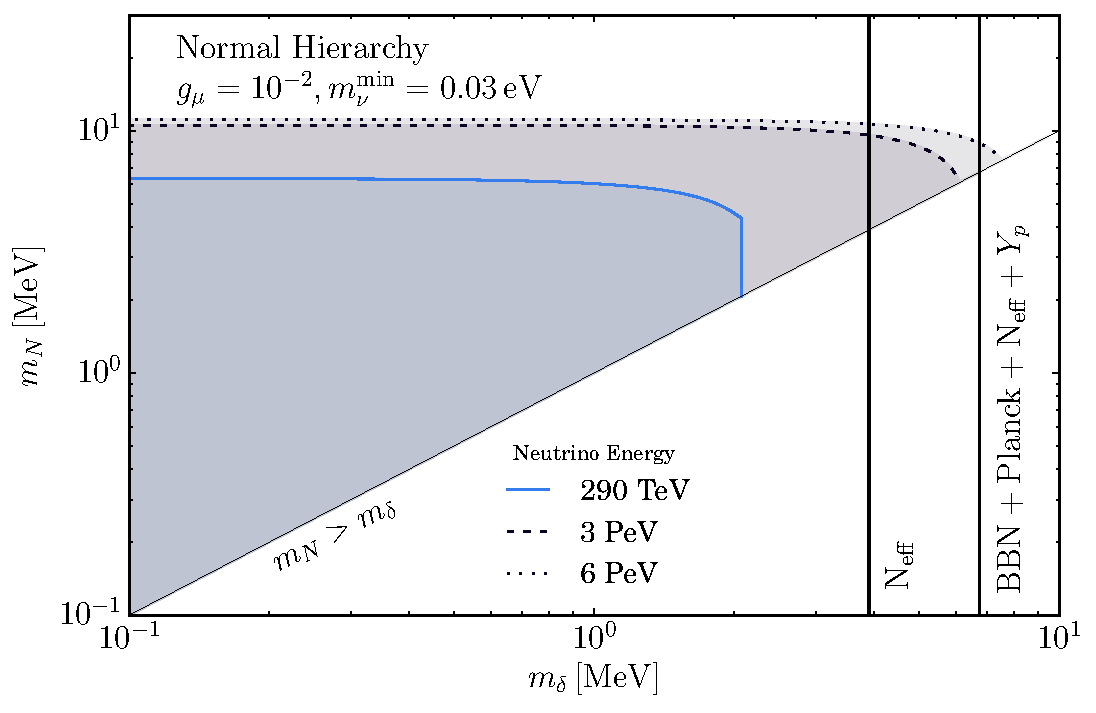
\includegraphics[width=.8\textwidth]{mpmnconstraints.pdf}
 \caption{Expected constraints if higher energy neutrinos were detected from a source located at the same distance as TXS 0506+056. In this figure, we have taken $g_\mu = 10^{-2}$, $g_e = 0$, $g_\tau = 3 \times 10^{-1}$, and $m_\nu^{\mathrm{min}} = 0.03$ in the normal hierarchy. Shown vertically are CMB constraints \cite{Boehm} and CMB+BBN constraints \cite{Nollett2015}.}
 \label{fig:mpmn}
\end{figure}

We now turn to comparing our constraints with those from cosmology, in particular it turns out that the contribution to the neutrino temperature in the early Universe due to the interaction of the thermal bath with these light dark matter candidates is significant.  Modification of the neutrino temperature affects the CMB, for example by changing the epoch of matter radiation equality.

In \cite{Boehm} the authors looked at the effect of a change in neutrino temperature on the CMB, while in \cite{Nollett2015}, the effect of a different temperature of neutrinos on both the CMB and BBN were also taken into account (see also \cite{Escudero2019}. These two studies lead to a stronger constraint on the mass of scalar dark matter coupled to the neutrino sector than the limits we are currently able to obtain from IceCube.  As an aside, it is interesting that two constraint from such radically different astrophysical environments lead to similar numbers. In Figure \ref{fig:mpmn} we plot these constraints neglecting any dependence on the mediator mass and we estimate what energy neutrino we would have to observe from TXS 0506+056 in order to get a stronger constraint. The CMB and BBN constraints on the model change the acceptable region where mass generation in this way is acceptable but leave enough parameter space open to not rule out the mechanism all together.


Taking a slightly bigger picture view, this shows that the exciting new data from IceCube can lead to new constraints on physics beyond the standard model, as shown also in \cite{Kelly}. Ultimately detecting neutrinos is difficult, and this analysis will only improve with more observations. As the IceCube experiment runs longer and longer, more regions of parameter space can be tested, as discussed in Section \ref{sec:cmbconstraints} and illustrated in Figure \ref{fig:mpmn}. It would also allow for a statistical treatment of the phenomenon which is simply not appropriate here with a single event.

To extend the analysis, we should consider the splitting of the mass eigenstates. In the case that there was a very large mass splitting, the constraints would weaken slightly as the centre of mass energy may not be sufficient to excite all the interaction modes. This will ultimately only lead to a maximum of a factor of $3$ difference in the mean free path, which is subdominant compared to changes in e.g. the coupling constants.

\vspace{-0.2cm}

\section{Discussion}\label{sec:conclusion}

To summarise, we have considered new constraints on an effective theory that links Dark Matter and neutrino masses. Within this framework, we used the IceCube event 170922A to obtain bounds on the interaction of neutrinos with MeV scalar dark matter. Our constraints are an order of magnitude improvement on the constraints which can be obtained by Kaon decay and are competitive with those coming from CMB and BBN, although not yet quite as strong.  We have calculated the energy of neutrinos that would need to be detected in order to beat the CMB and BBN constraint. Independent of the performance, it indicates the utility of IceCubce as a probe of fundamental physics. We also extended the analysis in \cite{Kelly} regarding the blazar dynamics to address some of the subtleties that arise in the higher energy neutrino regime. We argued that the various astrophysical papers \cite{Padovani2018, Padovani2019, Keivani2018} support the conclusion that the mean free path was a suitable comparison parameter in a fairly model independent fashion.

In terms of the assumptions contained in our analysis, we would like to ultimately relax the mass splitting assumption, although as noted above, we do not believe this would make a significant difference. For a very precise calculation, we should also include the effects of neutrino clustering for example.

Looking forward, the biggest improvement will be found once IceCube observes more ultra high energy astrophysical neutrinos from sources gigaparsecs away. The coincidence of the centre of mass energy and the scalar mass makes this sort of event the perfect setting to consider the effective model. Further work could then implement a fuller statistical analysis and provide confidence intervals on the bounds. One could also place similar constraints on the remaining portion of the models detailed in \cite{BoehmPascoli}. Moreover, one could look to investigate the amount of data required for clear discrimination between models. This would be a valuable step towards making this method of constraint a precise tool.


\clearpage

\begin{figure}[t]
 \centering
 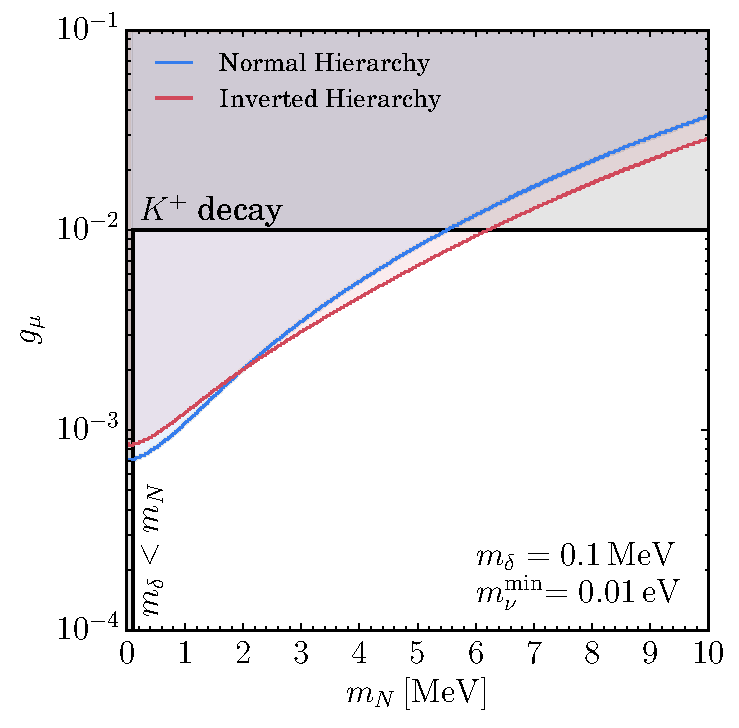
\includegraphics[width=.48\textwidth]{1.pdf}\quad
 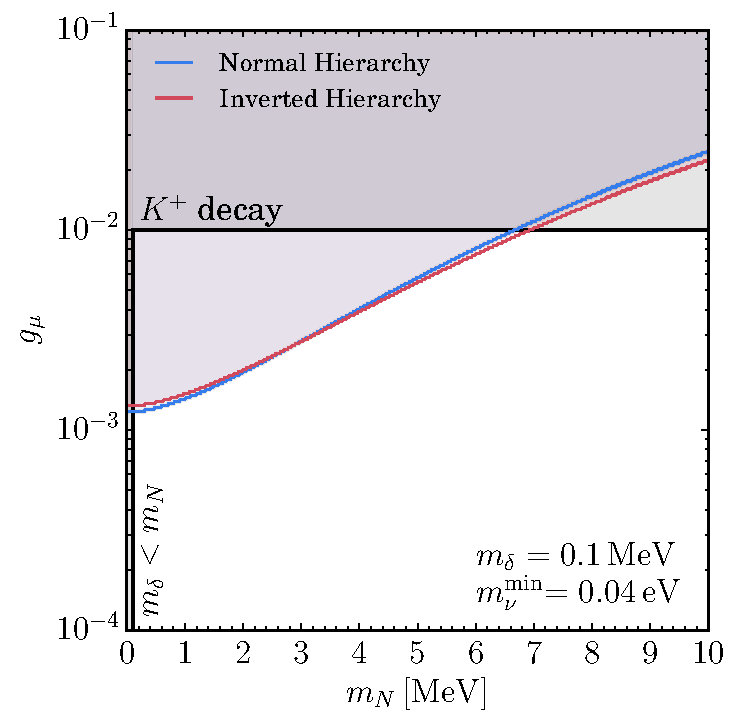
\includegraphics[width=.48\textwidth]{3.pdf}

 \medskip

 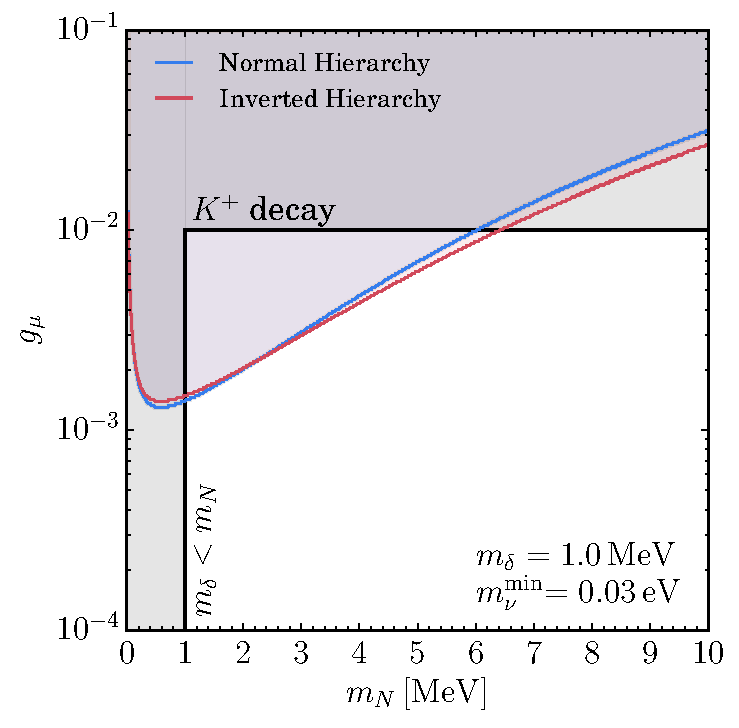
\includegraphics[width=.48\textwidth]{8.pdf}\quad
 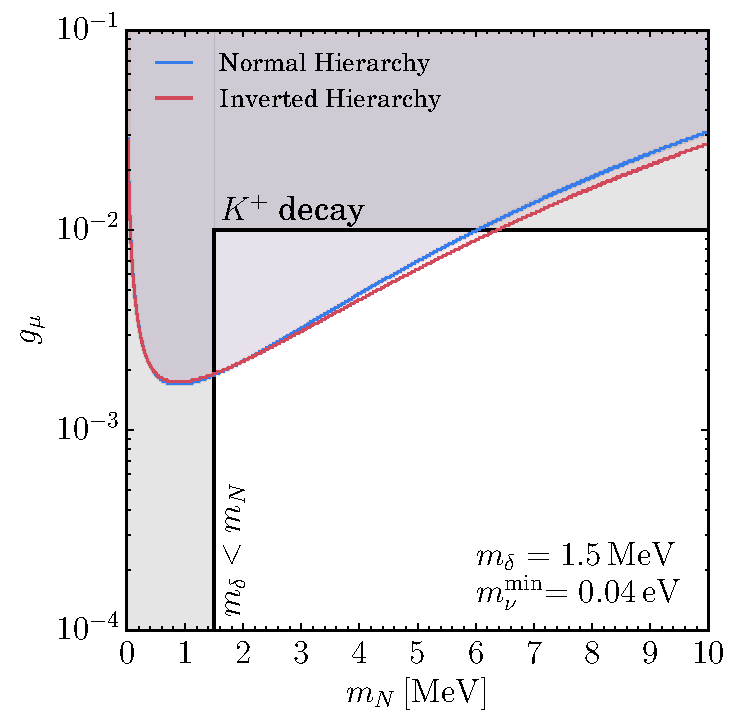
\includegraphics[width=.48\textwidth]{11.pdf}
 \caption{Selection of constraint plots for the case of complex scalar dark matter. In each plot, $g_e = 0$, $g_\tau = 3 \times 10^{-1}$, and the shaded regions are those that are ruled out by the mean free path constraints.}
 \label{fig:main}
\end{figure}
\clearpage